\documentclass[12pt]{article}

\usepackage{graphicx} 
\usepackage{tikz}   

\usetikzlibrary{positioning}

\begin{document}

\begin{figure*}[!t]

\centering
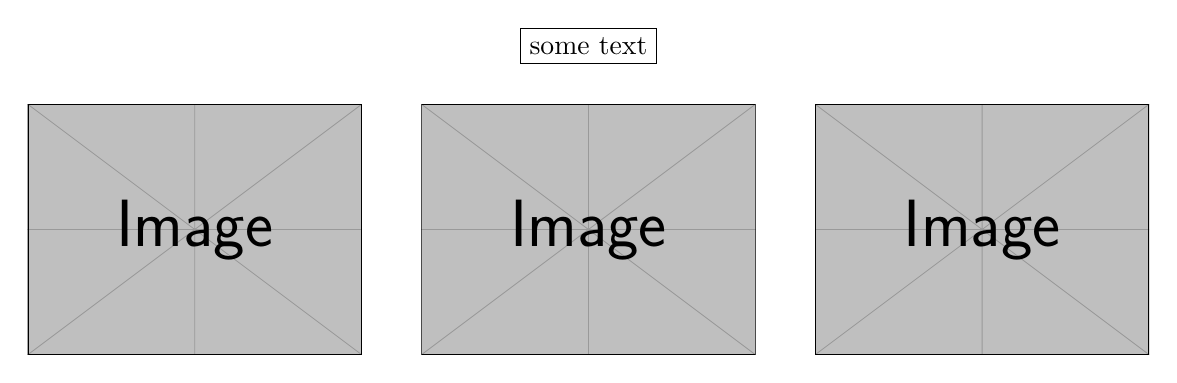
\begin{tikzpicture}

\node[anchor=south west,inner sep=0] (imagea) at (0,0) {\includegraphics[width=0.35\columnwidth]{example-image}};
\node[draw, align=center,above=0.5cm of imagea] {some text};

\node[anchor=south west,inner sep=0] at (-5,0) {\includegraphics[width=0.35\columnwidth]{example-image}};

\node[anchor=south west,inner sep=0] at (5,0) {\includegraphics[width=0.35\columnwidth]{example-image}};

\end{tikzpicture}
\end{figure*}

\end{document}